\section{Description of Findings}
\label{sec:findings}

Gapminder allows to answer many questions about the global world situation and its evolution over time.
We will try to give an answer to some of them:
\begin{itemize}
    \item What is the life expectation of the world population?
    \item What is the global trend of the average income?    
    \item What is the world situation in terms of population, average income, life expectation?
\end{itemize}


\subsection{Life Expectancy}
We can answer this question by using a chart of type ``maps'' and changing both the indicator shown as color and size to life expectancy.
We also reduce the size scale to avoid too many overlapping.
Each bubble represents a country and the position of the bubble represent its geographical location.
The resulting visualization is shown in \cref{fig:life-expectation}.
We use the most recent available data of $2015$.

\begin{figure}[h]
	\centering
	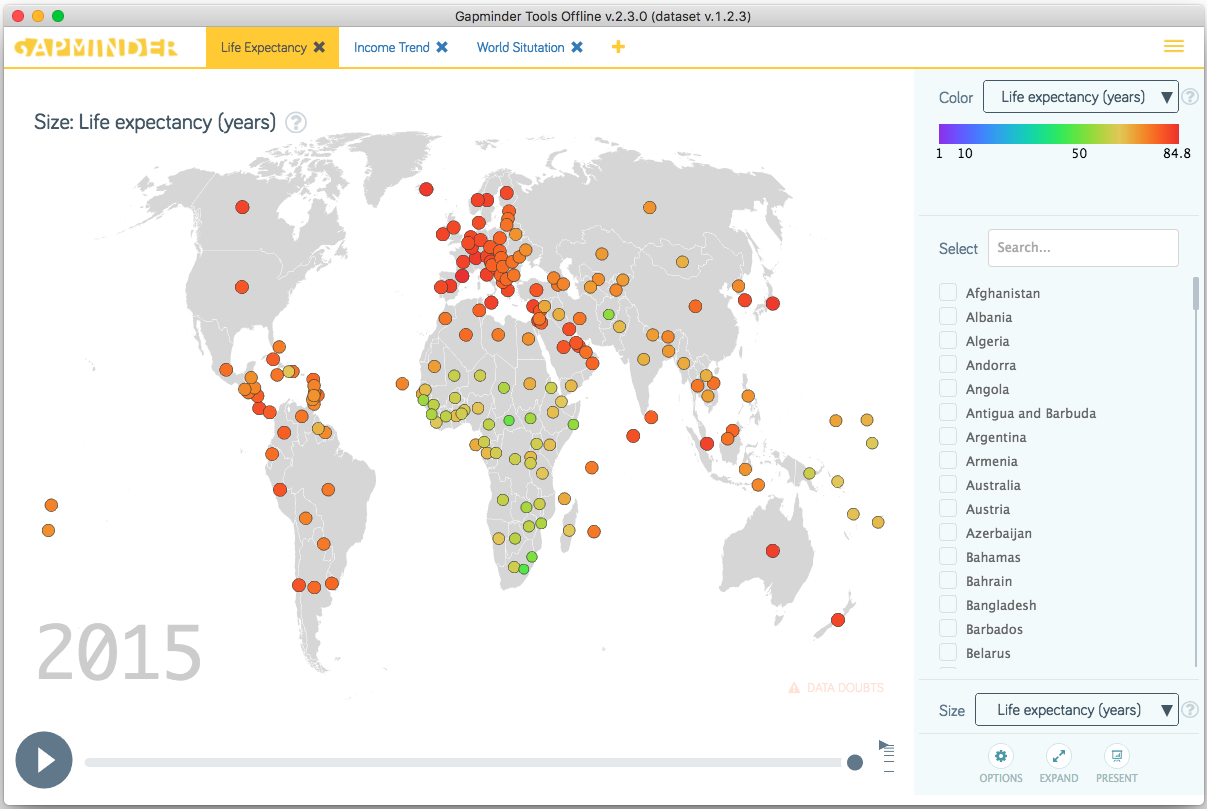
\includegraphics[width=0.95\columnwidth]{figures/life-expectancy}
	\caption{Life expectancy in $2005$ for the different countries of the world.}
	\label{fig:life-expectation}
\end{figure}

We can immediately notice groups of bubbles with different colors.
\begin{itemize}
	\item Bubbles in europe are red or dark orange, which indicates an average life expectation between $75$ (orange) and $85$ (red) years.	Countries in east europe tend to have a slightly lower life expectation that countries in the center and west.
	\item Countries in asia tend to have shorter life expectancy, between $65$ and $75$ years. There are however some exceptions: Japan, South Korea and Singapore have higher life expectations (respectively $83$, $81$ and $83$ years), while Afghanistan has a much shorter one, only $54$ years.
	\item New Zealand and Australia have high life expectations, while the small countries in the Pacific Ocean have quite much lower ones (between $60$ and $65$).
	\item Bubbles in Africa range from green to yellow / light orange. This indicates life expectations between about $50$ and $65$ years. The situation is slightly better in the very north: life expectation here is between $70$ and $75$ years.
	\item Countries in america go from orange to red. Life expectation is quite high in the north (about $80$ years) and in the south (about $75$ years) and lower in the center (from $70$ to $75$ years).
\end{itemize}




\subsection{Income Trend}


\subsection{World Situation}

